\usetikzlibrary{decorations.pathreplacing}

\bigheading{Posters}

\authors{Marek Sommer}{Marek Sommer}{Marek Sommer}

\heading{Subtask solution}

The task statement specified that in $50\%$ of testcases,
	there holds $n, m \le 1000$.
This subtask can be solved by considering each new poster separately.
So let's fix one of the new posters (and name it $P$), and let's find the answer for that poster.

For each poster, which hangs on the wall, we can substitute it with its intersection with $P$.
Those operations cannot change the final answer, because the parts of posters,
	which lay outside the poster $P$, wouldn't be counted anyway.
After these operations, the answer for poster $P$ is the total area
	covered by the changed posters.
From now on poster $P$ is useless.

To compute the answer, we will use the sweep line algorithm.
We will split each poster into two events -- the opening (left) and the closing (right) edge of the poster,
	and then we will process the events in order from left to right.

\begin{center}
	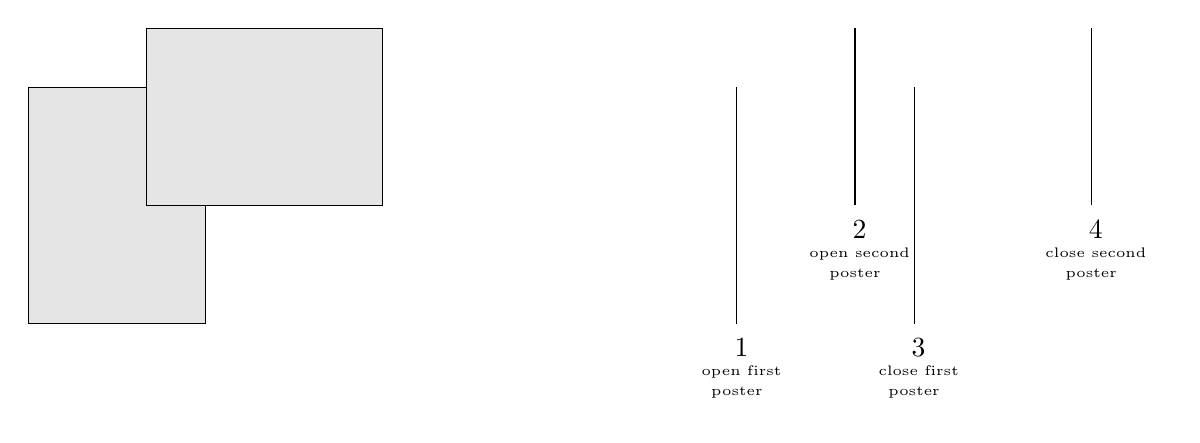
\begin{tikzpicture}[scale=0.75]
		\filldraw[gray!20] (0, 1) -- (3, 1) -- (3, 5) -- (0, 5) -- cycle;
		\draw (0, 1) -- (3, 1) -- (3, 5) -- (0, 5) -- cycle;
		\filldraw[gray!20] (2, 3) -- (6, 3) -- (6, 6) -- (2, 6) -- cycle;
		\draw (2, 3) -- (6, 3) -- (6, 6) -- (2, 6) -- cycle;

		\draw (9, 3) node {$\rightsquigarrow$};

		\draw (12, 1) node [below] {\begin{tabular}{c} \vspace{-5pt} $1$ \\ \vspace{-5pt} \tiny open first \\ \tiny poster \end{tabular}} -- (12, 5);
		\draw (14, 3) node [below] {\begin{tabular}{c} \vspace{-5pt} $2$ \\ \vspace{-5pt} \tiny open second \\ \tiny poster \end{tabular}} -- (14, 6);
		\draw (15, 1) node [below] {\begin{tabular}{c} \vspace{-5pt} $3$ \\ \vspace{-5pt} \tiny close first \\ \tiny poster \end{tabular}} -- (15, 5);
		\draw (18, 3) node [below] {\begin{tabular}{c} \vspace{-5pt} $4$ \\ \vspace{-5pt} \tiny close second \\ \tiny poster \end{tabular}} -- (18, 6);
	\end{tikzpicture}
\end{center}

After every event, we would like to know the length of the intersection of opened posters with vertical line from sweeping.
On the figures below, those intersections are marked with thick, dashed lines.

\begin{center}
	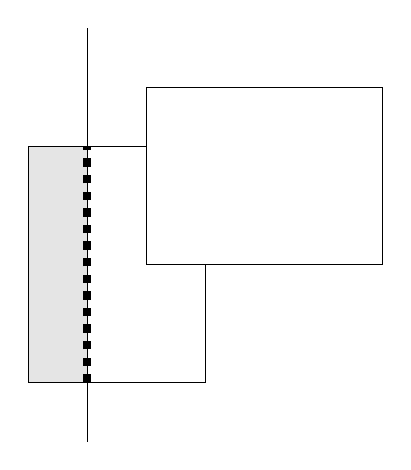
\begin{tikzpicture}[scale=0.75]
		\filldraw[gray!20] (0, 1) -- (1, 1) -- (1, 5) -- (0, 5) -- cycle;
		\draw (0, 1) -- (3, 1) -- (3, 5) -- (0, 5) -- cycle;
		\filldraw[white] (2, 3) -- (6, 3) -- (6, 6) -- (2, 6) -- cycle;
		\draw (2, 3) -- (6, 3) -- (6, 6) -- (2, 6) -- cycle;
		\draw (1, 0) -- (1, 7);
		\draw [line width=3, dashed] (1, 1) -- (1, 5);
	\end{tikzpicture}
	\qquad
	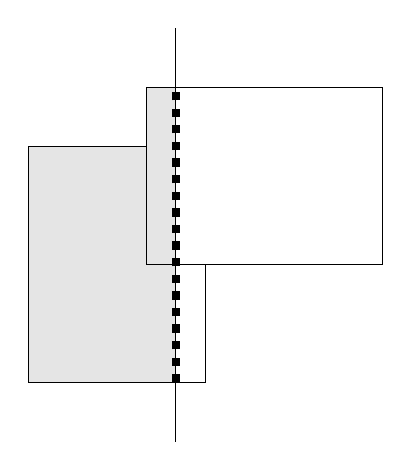
\begin{tikzpicture}[scale=0.75]
		\filldraw[gray!20] (0, 1) -- (2.5, 1) -- (2.5, 5) -- (0, 5) -- cycle;
		\draw (0, 1) -- (3, 1) -- (3, 5) -- (0, 5) -- cycle;
		\filldraw[white] (2, 3) -- (6, 3) -- (6, 6) -- (2, 6) -- cycle;
		\filldraw[gray!20] (2, 3) -- (2.5, 3) -- (2.5, 6) -- (2, 6) -- cycle;
		\draw (2, 3) -- (6, 3) -- (6, 6) -- (2, 6) -- cycle;
		\draw (2.5, 0) -- (2.5, 7);
		\draw [line width=3, dashed] (2.5, 1) -- (2.5, 6);
	\end{tikzpicture}
	\qquad
	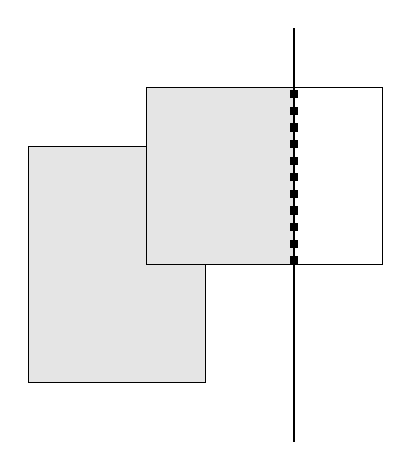
\begin{tikzpicture}[scale=0.75]
		\filldraw[gray!20] (0, 1) -- (3, 1) -- (3, 5) -- (0, 5) -- cycle;
		\draw (0, 1) -- (3, 1) -- (3, 5) -- (0, 5) -- cycle;
		\filldraw[gray!20] (2, 3) -- (4.5, 3) -- (4.5, 6) -- (2, 6) -- cycle;
		\draw (2, 3) -- (6, 3) -- (6, 6) -- (2, 6) -- cycle;
		\draw (4.5, 0) -- (4.5, 7);
		\draw [line width=3, dashed] (4.5, 3) -- (4.5, 6);
	\end{tikzpicture}
\end{center}

If we would be able to compute this value, then we could easily find the area covered by the posters,
	between two adjacent vertical lines.
To find this area, we could simply multiply the length of the intersection, by the distance between these lines.

\begin{center}
	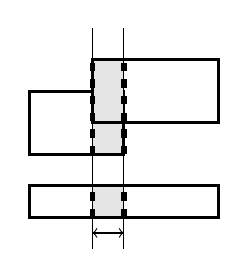
\begin{tikzpicture}[scale=0.4]
		\filldraw[gray!20] (2, 2) -- (3, 2) -- (3, 4) -- (2, 4) -- cycle;
		\draw [line width=1.2] (0, 2) -- (3, 2) -- (3, 4) -- (0, 4) -- cycle;
		\filldraw[gray!20] (2, 3) -- (3, 3) -- (3, 5) -- (2, 5) -- cycle;
		\draw [line width=1.2] (2, 3) -- (6, 3) -- (6, 5) -- (2, 5) -- cycle;
		\filldraw[gray!20] (2, 0) -- (3, 0) -- (3, 1) -- (2, 1) -- cycle;
		\draw [line width=1.2] (0, 0) -- (6, 0) -- (6, 1) -- (0, 1) -- cycle;

		\draw [line width=2, dashed] (2, 0) -- (2, 1);
		\draw [line width=2, dashed] (3, 0) -- (3, 1);
		\draw [line width=2, dashed] (2, 2) -- (2, 5);
		\draw [line width=2, dashed] (3, 2) -- (3, 5);

		\draw (2, -1) -- (2, 6);
		\draw (3, -1) -- (3, 6);

		\draw [<->] (2, -0.5) -- (3, -0.5);
	\end{tikzpicture}
\end{center}

We will build a segment tree, which will count the length of this intersection.
The leafs in the segment tree will represent the spaces between $y$ coordinates, which belong to any poster.
The other vertices will represent the spaces, which belong to their sons.

\begin{center}
	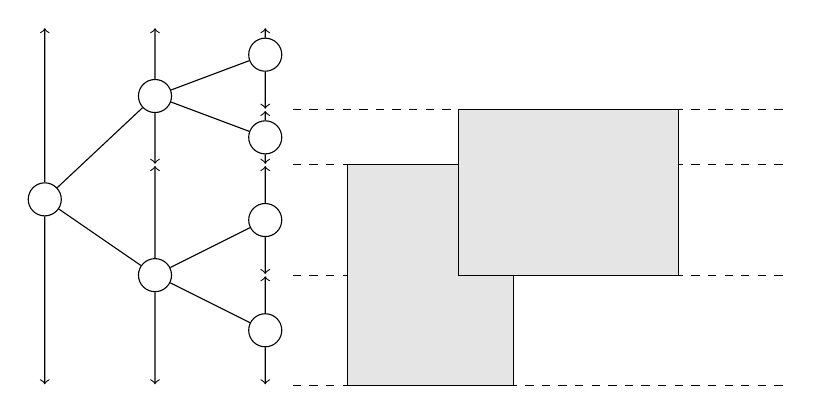
\begin{tikzpicture}[scale=0.7]
		\draw [dashed] (-1, 1) -- (8, 1);
		\draw [dashed] (-1, 3) -- (8, 3);
		\draw [dashed] (-1, 5) -- (8, 5);
		\draw [dashed] (-1, 6) -- (8, 6);

		\filldraw[gray!20] (0, 1) -- (3, 1) -- (3, 5) -- (0, 5) -- cycle;
		\draw (0, 1) -- (3, 1) -- (3, 5) -- (0, 5) -- cycle;
		\filldraw[gray!20] (2, 3) -- (6, 3) -- (6, 6) -- (2, 6) -- cycle;
		\draw (2, 3) -- (6, 3) -- (6, 6) -- (2, 6) -- cycle;

		\node (1) at (-5.5, 4.375) {};
		\node (2) at (-3.5, 3) {};
		\node (3) at (-3.5, 6.25) {};
		\node (4) at (-1.5, 2) {};
		\node (5) at (-1.5, 4) {};
		\node (6) at (-1.5, 5.5) {};
		\node (7) at (-1.5, 7) {};

		\draw (1) -- (2);
		\draw (1) -- (3);
		\draw (2) -- (4);
		\draw (2) -- (5);
		\draw (3) -- (6);
		\draw (3) -- (7);

		\draw [->] (1) -- ++(0, 3.105);
		\draw [->] (1) -- ++(0, -3.355);
		\draw [->] (2) -- ++(0, 1.98);
		\draw [->] (2) -- ++(0, -1.98);
		\draw [->] (3) -- ++(0, 1.23);
		\draw [->] (3) -- ++(0, -1.23);
		\draw [->] (4) -- ++(0, 0.98);
		\draw [->] (4) -- ++(0, -0.98);
		\draw [->] (5) -- ++(0, 0.98);
		\draw [->] (5) -- ++(0, -0.98);
		\draw [->] (6) -- ++(0, 0.48);
		\draw [->] (6) -- ++(0, -0.48);
		\draw [->] (7) -- ++(0, 0.48);
		\draw [->] (7) -- ++(0, -0.98);

		\filldraw [white] (1) circle (0.3);
		\filldraw [white] (2) circle (0.3);
		\filldraw [white] (3) circle (0.3);
		\filldraw [white] (4) circle (0.3);
		\filldraw [white] (5) circle (0.3);
		\filldraw [white] (6) circle (0.3);
		\filldraw [white] (7) circle (0.3);

		\draw (1) circle (0.3);
		\draw (2) circle (0.3);
		\draw (3) circle (0.3);
		\draw (4) circle (0.3);
		\draw (5) circle (0.3);
		\draw (6) circle (0.3);
		\draw (7) circle (0.3);
	\end{tikzpicture}
\end{center}

In each vertex we should hold some information about the range it represents.

First of all, the length of a range should be known.
It is easy to find such a value for every leaf, and for other vertices we could compute it,
	by adding the lengths of both sons.
Let's call this value \texttt{length}.

The second value stored in a vertex is an indicator whether the whole range
	(which is represented by this vertex) lies inside any opened rectangle.
If this value is grater than zero, then it means that there is such a rectangle,
	but if the value is equal to zero, than it does not necessarily mean that there is no such rectangle,
	because this value could be grater than zero in any ancestor of that vertex.

The third value would be the one we are looking for
	-- the length of the intersection of opened rectangles with the sweeping line.
We will call it a \texttt{covered} value.

Updating this values on our segment tree is easy.
If we meet an opening (closing) edge of a rectangle, then we should find the vertices,
	whose ranges cover the whole edge of that rectangle.
Then we should increase (decrease) the second value in each of these vertices,
	and then we should update the \texttt{covered} value in every node on the path
	from each of those vertices to the root.
If we try to update the \texttt{covered} value in vertex $v$, than we should consider some cases:
\begin{itemize}
	\item If $v$ is a leaf:
		\begin{itemize}
			\item If second value in $v$ is equal to $0$, then the \texttt{covered} value is equal to $0$.
			\item If second value in $v$ is grater than $0$, then the \texttt{covered} value
				is equal to the length of the range represented by $v$.
		\end{itemize}
	\item If $v$ is not a leaf:
		\begin{itemize}
			\item If second value in $v$ is equal to $0$, then the \texttt{covered} value
				is equal to the sum of \texttt{covered} values of both sons.
			\item If second value in $v$ is grater than $0$, then the \texttt{covered} value
				is equal to the length of the range represented by $v$.
		\end{itemize}
\end{itemize}
This will not give us a correct \texttt{covered} value in every node,
	but the \texttt{covered} value in root will always be valid, after applying these updates.
We can also see that in next steps of our algorithm only the value from root will be needed.

That way, each tree update after opening or closing a rectangle is done in logarithmic time (in size of a tree).
Thus we can find the total area covered by $n$ rectangles in $O(n \log n)$ time.
If we consider each query separately, than we will get the $O(m n \log n)$ solution,
	which will give us $50\%$ of points.


\heading{Final solution}

To get $100\%$ points, we need to slightly modify our segment tree.
We would like to implement some new functionalities,
	which would allow us to consider all of the queries at the same time.

In the following description we will use a term ''time'' to name the $x$ coordinates.
For example, if we say ''now'', we will think about the current position of the sweeping line.

In our modified tree we would like to hold the total sum of the area covered by rectangles
	since the beginning of time till now (till the current sweep line position).
Of course, we will hold such a value in every vertex, and each vertex will
	hold information only about the area covered inside the horizontal strip
	determined by the vertex range.

We would like to be able to read the sum of these areas on the given range.
That would help us with queries, because if we split each query into the opening and closing edge,
	than we should only read the covered area from the beginning of time till the closing edge,
	and the covered area from the beginning of time till the opening edge,
	and then subtract those values
	to get the final answer.

Let's implement this total area feature.
In a vertex $v$ we should store two additional variables: \texttt{total\_area} and \texttt{last\_update}.
These values will mean that the last time we visited vertex $v$,
	was when the sweeping line was at the position \texttt{last\_update},
	and at that time, the total area (from the beginning of time) was equal to \texttt{total\_area}.

Let's say we now have time $T$, and we enter a vertex $v$.
We know that the current covered area since the beginning of time is equal to\footnote{
	This value is not totally valid, but we would like it to work like that.
	We will correct it later.
}:
\[
	v.\texttt{total\_area} + (T - v.\texttt{last\_update}) \cdot v.\texttt{covered}
\]
So, when we would like to enter any vertex in order to do something there
	(doesn't matter if we met an opening, or closing edge of a poster, or a query),
	we should increase the \texttt{total\_area} by the difference from the last update to now,
	and then we should set \texttt{last\_update} value to $T$.
We cannot leave this update for later, because the \texttt{covered} value might change in this vertex
	and then we won't be able to find the difference so easily.

There's still a small problem with this method.
Let's say that we update $v$ at time $t_1$, and $v.\texttt{covered}$ is equal to $0$
	(because there are no opened rectangles there).
Then, at time $t_2$, we open a rectangle, and during that operation
	we update some vertices \textbf{above} $v$.
The range represented by $v$ is covered by this rectangle, but we never reach $v$,
	because we stopped in any ancestor of $v$.
Then we close this rectangle at time $t_3$, and we still don't reach $v$.
If we finally visit $v$ at time $t_4$ we would like to update $v.\texttt{total\_area}$,
	but with the previous formula we would add $(t_4 - t_1) \cdot 0$,
	because the \texttt{covered} value is equal to $0$.
We see that this value is not correct, because since $t_2$, until $t_3$,
	there was a rectangle covering $v$'s range.
Thus, we should add $(t_3-t_2) \cdot v.\texttt{length}$ instead.

In each vertex we should hold an information about the total time,
	when the range was fully covered since the last update.
We can call this value \texttt{fully\_covered}.
Let's say that we enter the vertex $v$ at time $T$ and we try to update it.
We should increase the \texttt{total\_area} value by:
\[
	(T - v.\texttt{last\_update} - v.\texttt{fully\_covered}) \cdot v.\texttt{covered}
		+ v.\texttt{fully\_covered} \cdot v.\texttt{length}
\]
And then, we should set \texttt{last\_update} to $T$ and \texttt{fully\_covered} to $0$.

To maintain the \texttt{fully\_covered} value, we should also increase vertex's both sons' \texttt{fully\_covered} value
	with $v.\texttt{fully\_covered}$, because if $v$ was covered,
	then all of its descendants were also covered during that time.
If the ''second value'' in $v$ is grater than $0$ we should also increase the sons' \texttt{fully\_covered}
	value by the time that passed from $v.\texttt{last\_update}$ until $T$,
	without counting the $v.\texttt{fully\_covered}$ time.

Such updating allows us to maintain the total covered area in \textbf{every} vertex.
This leads us to an $O((n+m) \log (n+m))$ solution.
